% ============================================================
%  7.6. DESPLIEGUE  -- parte del capítulo 7
%  ------------------------------------------------------------
%  Archivo separado para que cada fase de CRISP-DM se pueda
%  editar y compilar por separado. Solo contenido: el formato,
%  los rótulos y las referencias los resuelve el preámbulo.
%  Los \label originales se conservan sin cambios.
% ============================================================
\section{Despliegue}
\label{sec:despliegue}

Esta sección documenta la sexta fase de CRISP-DM, construida sobre el modelo final de la
sección~\ref{sec:seleccion-final} y la evaluación de la
sección~\ref{sec:evaluacion-resultados}.

\subsection{Caso de uso en un contexto real}

El resultado del proyecto es una \textbf{capa analítica de priorización territorial}: demanda
esperada de consultas por celda H3 y semana, cruzada con la brecha de cobertura GTFS. No
sustituye la decisión humana de planificación de rutas: implica error real por celda (MAE de
10,19, o 5,91 en semanas completas, sección~\ref{sec:semanas-parciales}), y H2
(sección~\ref{sec:contraste-hipotesis}) mostró que la ventaja del modelo se concentra en
celdas de alta demanda, no en todas. El uso concreto propuesto es priorizar, dentro del
proceso de mapeo voluntario de rutas de Trufi App descrito en la
sección~\ref{sec:comprension-negocio}, qué celdas de baja cobertura conviene atender primero.

\subsection{Prototipo y arquitectura}

Se construyó un \textbf{servicio real y ejecutable}, no solo un diagrama: \var{src/trufi_ds/api.py}
(FastAPI), que carga el modelo Random Forest final y reconstruye, para cualquier celda, el
vector de variables de la semana siguiente a la última observada, con exactamente la misma
lógica de ingeniería de características usada en el entrenamiento
(sección~\ref{sec:seleccion-algoritmos}). Expone \texttt{GET /predict?cell=...} para una
celda individual y \texttt{GET /cells/top?n=...} para el caso de uso de priorización. La guía
UMSS admite una propuesta fundamentada cuando no hay despliegue completo; un prototipo
verificable localmente satisface el requisito con evidencia y no solo con intención.

\begin{figure}[htbp]
  \centering
  \caption{Arquitectura de actualización y consumo del modelo}
  \label{fig:arquitectura}
  
\includegraphics[width=0.85\textwidth]{imagenes/logo_facultad.png}
  \fuente{Elaboración propia. Diagrama descrito textualmente a continuación; el flujo
  completo (Mermaid) está documentado en \var{reports/05_deployment/01_deployment_architecture.md}.}
\end{figure}

El flujo conecta componentes que ya existen como código en este repositorio, sin
componentes hipotéticos: el feed GTFS (actualización semanal, \var{run_update_pipeline.py})
y las exportaciones de consultas alimentan el cálculo de cobertura
(sección~\ref{sec:cobertura-gtfs}) y la tabla de indicadores
(sección~\ref{sec:tabla-indicadores}); de ahí se derivan, por un lado, el reentrenamiento
trimestral del modelo (\var{18_model_training.py}) y, por otro, la reconstrucción del
panel de features que consume el servicio de predicción; el plan de monitoreo
(sección~\ref{sec:monitoreo}) vigila el servicio en producción.

\subsection{Consumo del modelo}

Los siguientes son ejemplos reales, obtenidos ejecutando el servicio contra los datos y el
modelo actuales del repositorio --no respuestas hipotéticas--, incluido un caso de error
controlado.

\begin{table}[htbp]
  \centering
  \caption{Ejemplos de consumo del prototipo de predicción}
  \label{tab:ejemplos-api}
  \interlineadoSimple
  \begin{tabularx}{\textwidth}{@{}p{0.34\textwidth}X@{}}
    \toprule
    \textbf{Solicitud} & \textbf{Respuesta (resumida)} \\
    \midrule
    \texttt{\small GET /predict?\allowbreak cell=\allowbreak 888b2c8ae5fffff}\newline (celda central, alta demanda) &
      Demanda predicha para 2024-W24: 737,0 consultas; distancia al centro 2,2~km; sin
      brecha de cobertura (\var{pct_uncovered_orig}$=0$) \\
    \texttt{\small GET /predict?\allowbreak cell=\allowbreak 888b2c80d5fffff}\newline (celda periférica, baja demanda) &
      Demanda predicha: 8,2 consultas; distancia al centro 17,2~km \\
    \texttt{\small GET /predict?\allowbreak cell=\allowbreak celda\_inexistente} &
      HTTP 404, error controlado: \textit{``Celda desconocida (sin historial)''} \\
    \texttt{\small GET /cells/top?\allowbreak n=5} &
      Devuelve las 5 celdas de mayor demanda predicha (782,0 a 732,3 consultas), calculadas
      en vivo sobre la última semana observada \\
    \bottomrule
  \end{tabularx}
  \fuente{Elaboración propia, a partir de \var{24_deployment_architecture.py} ---
  \var{reports/05_deployment/01_deployment_architecture.md}.}
\end{table}

Construir y ejercitar el prototipo --no solo describirlo-- expuso una limitación operativa
real: la última semana del dataset, 2024-W23, es en sí misma una de las semanas parciales
documentadas en la sección~\ref{sec:semanas-parciales}, por lo que la primera predicción en
vivo heredaría un \texttt{lag1} artificialmente bajo para todas las celdas. La mitigación
propuesta es completar (\textit{backfill}) esa semana con datos reales antes de servir la
primera predicción en producción, o aceptar explícitamente un primer ciclo de error elevado.

\subsection{Priorización territorial: celdas a mapear}
\label{sec:priorizacion}

La regla de decisión propuesta ordena las celdas por \textbf{demanda no resuelta}: el
producto de la demanda semanal esperada por la tasa de no cobertura de cada celda, usando la
mediana de cobertura de cada celda en el período de \emph{entrenamiento} --nunca el valor de
la semana objetivo, que sería conocer el futuro. Ordenar por demanda bruta, en cambio, no
sirve como regla de priorización: devuelve las cinco celdas más consultadas del área
metropolitana, todas ellas ya con tasa de no cobertura nula --intervenirlas no aportaría
nada. Cruzar demanda con brecha de cobertura es lo que convierte el ranking en una decisión
accionable.

\begin{figure}[htbp]
  \centering
  \caption{Cuadrantes de priorización: demanda esperada vs. cobertura GTFS}
  \label{fig:cuadrantes-priorizacion}
  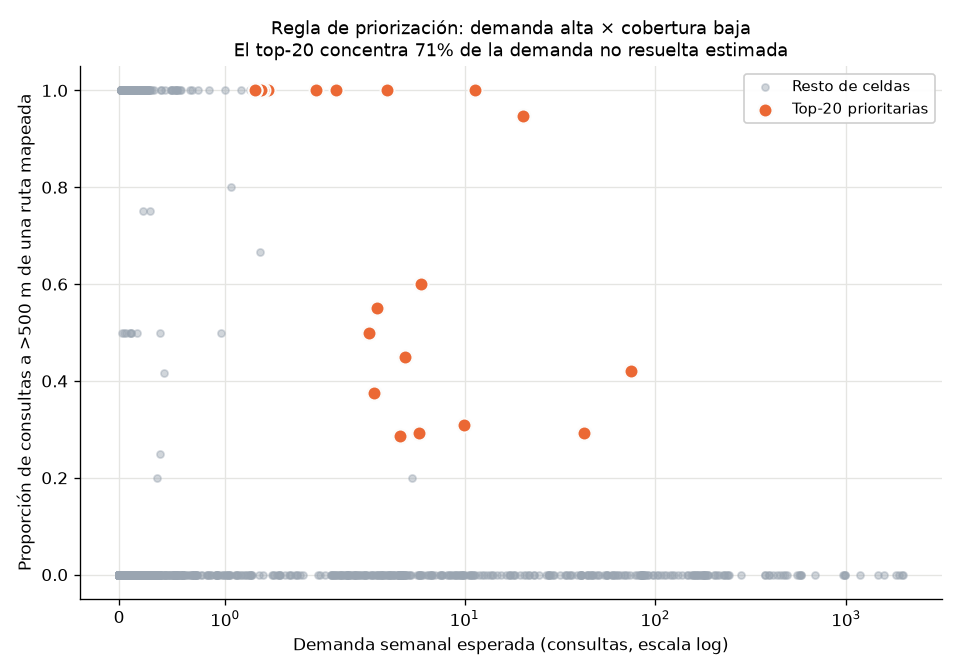
\includegraphics[width=0.75\textwidth]{imagenes/fig_priority_quadrants.png}
  \fuente{Elaboración propia, a partir de \var{27_priority_cells.py} ---
  \var{reports/05_deployment/03_priority_cells.md}.}
\end{figure}

El top-20 de celdas prioritarias concentra el \textbf{70,5~\%} de toda la demanda no resuelta
estimada del área metropolitana. Consistente con la figura, esas celdas \textbf{no son las de
mayor demanda absoluta}: son celdas de demanda baja o media (entre 1 y 74 consultas/semana)
mal cubiertas por el mapeo actual --la misma conclusión de H1 vista desde la decisión
operativa. Dieciocho de las veinte celdas coinciden entre usar Random Forest o la media móvil
como estimador de demanda, coherente con la refutación de la
sección~\ref{sec:sirve-para-priorizar}: el valor de esta tabla está en cruzar demanda con
cobertura, no en el estimador que produce la demanda.

\subsection{Monitoreo y reentrenamiento}
\label{sec:monitoreo}

Los umbrales de monitoreo se derivan de la distribución real de error y volumen de este
proyecto, no de valores convencionales.

\begin{table}[htbp]
  \centering
  \caption{Plan de monitoreo y reentrenamiento}
  \label{tab:monitoreo}
  \interlineadoSimple
  \begin{tabularx}{\textwidth}{@{}p{0.30\textwidth}p{0.16\textwidth}X@{}}
    \toprule
    \textbf{Métrica} & \textbf{Frecuencia} & \textbf{Umbral / acción} \\
    \midrule
    Volumen semanal total de consultas & Semanal & $<10.041$ consultas (30~\% de la mediana
    de las últimas 13 semanas no parciales) $\to$ marcar la semana como incompleta y
    excluirla del cálculo de \texttt{lag1} \\
    MAE semanal (predicción vs. real) & Semanal & $>11{,}64$ consultas (media $+\ 2\sigma$
    de las 6 semanas de prueba limpias) durante 2 semanas consecutivas $\to$ reentrenar antes
    del ciclo trimestral \\
    Actualización del feed GTFS & Semanal & Automática, ya implementada
    (\var{run_update_pipeline.py}) \\
    Reentrenamiento completo & Trimestral & Alineado con la ventana de 13 semanas de la
    validación cruzada (sección~\ref{sec:proceso-entrenamiento}) \\
    \bottomrule
  \end{tabularx}
  \fuente{Elaboración propia, a partir de \var{25_monitoring_plan.py} ---
  \var{reports/05_deployment/02_monitoring_plan.md}.}
\end{table}

El chequeo de completitud de datos existe \emph{porque} la sección~\ref{sec:semanas-parciales}
encontró el problema que previene: con este piso, las semanas 2024-W18 (909 consultas) y
2024-W23 (1.367 consultas) se habrían marcado automáticamente como incompletas en lugar de
descubrirse meses después durante el análisis de errores.

\subsection{Alcance del despliegue y trabajo pendiente}

No se despliega el servicio a un dominio público ni se automatiza el reentrenamiento con un
orquestador real (Airflow o un programador de tareas en un servidor productivo) --fuera del
alcance declarado de este trabajo (capítulo~\ref{cap:alcance}). Lo que se entrega en su lugar
es un prototipo funcional y verificable localmente, una arquitectura documentada que conecta
código ya existente, umbrales de monitoreo cuantificados a partir de los propios resultados
del proyecto, y una limitación operativa real --no hipotética-- descubierta al construir el
prototipo, con su mitigación propuesta. Antes de un uso productivo más allá de lo local
harían falta, como mínimo, autenticación, límites de tasa, un orquestador para el
reentrenamiento periódico y pruebas automatizadas de regresión sobre las métricas del modelo.
